\documentclass[main.tex]{subfiles}

\pagestyle{fancy}
\fancyhf{}
\fancyhead[LE]{\makebox[\pageoffset][l]{\bfseries\thepage}\bfseries\leftmark}
\fancyhead[RO]{\bfseries\rightmark\makebox[\pageoffset][r]{\bfseries\thepage}}

\begin{document}

\section*{Goal}
Today we will continue our discussion of angular motion this time looking at the counterpart to momentum, angular momentum. We will also investigate moments of inertia further which we introduced in Chapter~\ref{chap:Torque}. In our experiment we will use the conservation of angular momentum to calculate the moment of inertia of several different objects.

\section*{Equipment}
\begin{itemize}
\item
PASCO Capstone Software
\item
850 Universal Interface (850UI)
\item
Rotary Motion Sensor
\item
Silver Disk, White Disk, Rod with masses, Odd-Shaped Object
\item
Triple-beam Balance
\end{itemize}•

\section*{Theory}
The last rotational quantity we want to investigate in this class is angular momentum. As can be assumed angular momentum $\mathbf{L}$ is related to linear momentum $\mathbf{p}$ in the same way that torque is related to force,
\begin{equation} \label{eq:VectAngMom}
\mathbf{L}=\mathbf{r} \times \mathbf{p}.
\end{equation}
As it was with torque (Equation~\eqref{eq:MagTorque}) the magnitude of angular momentum is,
\begin{equation}\label{eq:MagAngMom}
L=rp\sin\theta,
\end{equation}
and if $\theta=\pi/2$ then Equation~\eqref{eq:MagAngMom} simplifies to 
\begin{equation} \label{eq:Lmvr}
L=rp=mvr
\end{equation}
We can however write an expression completely in terms of angular quantities which will be more useful to us given our equipment. Like we did in Chapter~\ref{chap:Torque}, let us consider our body as a collection of small pieces. Each piece of mass $m_i$ will rotate around a circle centered on the axis of rotation with a velocity $v_i.$ This tangential velocity vector $\mathbf{v}_i$ will always be perpendicular to a position vector $\mathbf{r}_i$ as we saw in Chapter~\ref{chap:Cen_Force}. We also know from Chapter~\ref{chap:Cen_Force} that $v_i=r_i\omega.$ Therefore we can write Equation~\eqref{eq:Lmvr} as,
\begin{equation}
L_i=m_i(r_i\omega)r_i=m_ir_i^2\omega.
\end{equation}
Now the total angular momentum $L$ of the body will be the sum of all the individual angular momenta $L_i$ of the particles,
\begin{equation}
L=\sum L_i=\left(\sum m_ir_i^2\right)\omega=I\omega,
\end{equation}
where we define $I=\sum m_ir_i^2$ to be the moment of inertia of the body and describes how mass is distributed around a rotating body. 
\begin{table}
\begin{tabular}{|p{0.3\textwidth}|c|c|}
\hline
\textbf{Point Mass} (at a distance $r$ from the axis of rotation) & 
\raisebox{-0.6\height}{
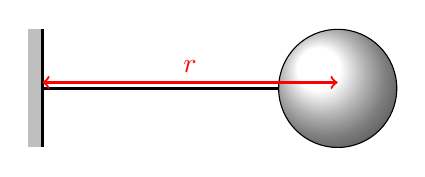
\begin{tikzpicture}[scale=0.75]
	\fill[ball color=white!10] (0,0) circle (1cm);
	\draw (0,0) circle (1cm);
	\draw[very thick] (-1,0) -- (-5,0);
	\fill[color=lightgray] (-5,1) --(-5,-1) -- (-5.25,-1) -- (-5.25,1) -- cycle;
	\draw[very thick] (-5,1) -- (-5,-1);
	\draw[<->,red,thick] (0,0.1) -- (-5,0.1) node [midway, above] {$r$};
\end{tikzpicture}
}
& $I=mr^2$\\
\hline
\textbf{Solid Disk} (of radius $r$ rotating about an axis through the center of the disk) &
\raisebox{-0.7\height}{
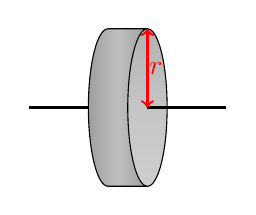
\begin{tikzpicture}[scale=0.5,rotate=-90]
	\fill[left color=gray!50!black,right color=gray!50!black,middle color=gray!50,shading=axis,opacity=0.25] (2,0) -- (2,1) arc (360:180:2cm and 0.5cm) -- (-2,0) arc (180:360:2cm and 0.5cm);
	\fill[top color=gray!90!,bottom color=gray!2,middle color=gray!30,shading=axis,opacity=0.25] (0,1) circle (2cm and 0.5cm);
	\draw (-2,1) -- (-2,0) arc (180:360:2cm and 0.5cm) -- (2,1) ++ (-2,0) circle (2cm and 0.5cm);
	\draw[very thick] (0,-2) -- (0,-0.5);
	\draw[very thick] (0,1) -- (0,3);
	\draw[<->,red,thick] (0,1) -- (-2,1) node [midway,right,xshift=-3pt] {$r$};
\end{tikzpicture}
}
& $I=\frac{1}{2}mr^2$\\
\hline
\textbf{Thin Rod} (of length $l$ rotating about an axis perpendicular to the rod and through its center) &
\raisebox{-0.8\height}{
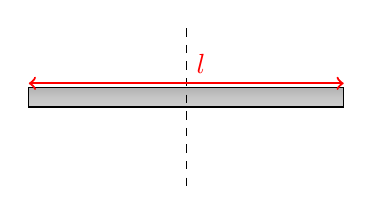
\begin{tikzpicture}[scale=1]
	\fill[top color=gray!90!,bottom color=gray!2,middle color=gray!30,shading=axis,opacity=0.25] (-2,0) rectangle (2,0.25);
	\draw (-2,0) rectangle (2,0.25);
	\draw[dashed] (0,1) -- (0,-1);
	\draw[<->,red,thick] (-2,0.3) -- (2,0.3) node [midway, above right] {$l$};
\end{tikzpicture}
}
& $I=\frac{1}{12}ml^2$\\
\hline
\end{tabular}•
\caption{} \label{tab:I_obj}
\end{table}
Table~\ref{tab:I_obj} provides the formulas of the various geometries that we will use in our experiment. An important property about moments of inertia is that it is an additive quantity, meaning that if two or more objects are combined into one compound object then then total moment of inertia will be the sum of the individual moments.
\[
\sum I=I_1+I_2+\dotsb
\]
The \emph{conservation of angular momentum} states that in the absence of a net external torque, the total angular momentum of the system is constant. In our experiment we will be colliding two objects together. One object will always be the silver disk that is attached to the Rotary Motion Sensor. We will begin each collision by spinning the silver disk . Then we will drop onto it the second object, which will initially have zero angular velocity. All of our collisions will be perfectly inelastic collisions, meaning that the objects will stick together and rotate with the same final angular velocity. Thus,
\begin{align}
L_i&=L_f \nonumber\\
I_1\omega_i &= (I_1+I_2)\omega_f. \label{eq:ConsAngMom}
\end{align}•

For our experiment we will use the Rotary Motion Sensor (RMS) to measure the angular velocity of our system before and after we drop an object on the rotating silver disk.
\begin{enumerate}
\item
Open Capstone.
\item
Connect the RMS to the 850UI then setup Capstone to record from the sensor (click on the left-most port that the sensor is plugged into).
\item
Create a graph of Angular Velocity vs Time.
\item
Mount the RMS on the vertical rod in the table so that the disks will be on top.
\end{enumerate}•

\subsection*{Procedure}
\begin{enumerate}
\item
Measure the mass of the silver disk and record it. Measure the diameter of the silver disk three different times from different locations on the disk and record the average.
\item
Attach the silver disk to the RMS.
\item \label{step:AngMom_start}
Measure the mass of the white disk and record it. Measure the diameter three different times from different locations on the disk and record the average.
\item
Give the silver disk a spin. Click on the Record button to start data collection. After about 25 data points have been recorded, drop the white disk onto the spinning disk. After the collision click the Stop button to end the data collection. Rescale the data. If the collision on the graph is not sharp enough, then delete the data run and repeat this step.
\item \label{step:AngMom_end}
Click on the Coordinates Tool \includegraphics{Coordinates_Tool} and move it to the data point immediately before the collision. Record the angular velocity at this point in the data table as the initial angular velocity. Now move the tool to the data point immediately after the collision. Record the angular velocity at this point as the final angular velocity.
\item
Repeat steps~\ref{step:AngMom_start}--\ref{step:AngMom_end} with the silver disk and the rod. For the rod we will need to measure its mass (without the attached masses) and overall length, the mass of each attachable mass removed from the rod and the distance of each attachable mass from the center of rotation. Make sure the masses are attached at the outer set of holes.
\item
Repeat steps~\ref{step:AngMom_start}--\ref{step:AngMom_end} with the silver disk and the odd-shaped object. We only need to measure the mass of this object.
\item
Show all data runs with the Select Data Run button \includegraphics{Select_Data_Run}. \textbf{Print} out a copy of this graph for each group member.
\item[\emph{Optional:}]
Repeat steps~\ref{step:AngMom_start}--\ref{step:AngMom_end} with the silver disk and the rod. This time, move the masses to the inner set of holes on the rod. \textbf{Print} a copy of this run for each group member.
\end{enumerate}•

\subsection*{Analysis}
\begin{enumerate}
\item
We will use the white disk run to determine an experimental value for the moment of inertia of the silver disk and compare it to a theoretical value.
\begin{enumerate}
\item
Using the appropriate formula from Table~\ref{tab:I_obj}, calculate the theoretical moments of inertia for both disks.
\item
Using Equation~\eqref{eq:ConsAngMom} with the measured angular velocities and the theoretical moment of inertia for the \emph{white} disk calculate the moment of inertia for the \emph{silver} disk.
\item
Calculate the percent discrepancy of the experimental value for the moment of inertia of the silver disk with its theoretical value.
\end{enumerate}•
\item \label{step:Rod}
For the the rod/masses run we will determine an experimental value of the moment of inertia of the rod with attached masses and compare it to a theoretical value.
\begin{enumerate}
\item
To determine the theoretical moment of inertia of the rod with attached masses, we must first calculate the individual moments of inertia for each piece using the appropriate formulas from Table~\ref{tab:I_obj}. (We can treat the attachable masses as point masses.) Calculate the total moment of inertia by  summing each individual moment together.
\item
Using Equation~\eqref{eq:ConsAngMom} with the measured angular velocities and the \emph{experimental} moment of inertia for the silver disk, calculate the moment of inertia for the rod/masses.
\item
Calculate the percent discrepancy of the experimental moment of inertia of the rod/masses with its theoretical value.
\end{enumerate}•
\item
For the odd-shaped object run we will determine an experimental value for the moment of inertia for the object. We will then use this value to determine the \emph{radius of gyration}. If we consider revolving off center a point mass of the same mass as our object and with the same moment of inertia then the radius of gyration $r_G$ is given by,
\begin{equation} \label{eq:R_G}
I_{odd}=mr_G^2
\end{equation}
\begin{enumerate}
\item
Using Equation~\eqref{eq:ConsAngMom} with the measured angular velocities and the experimental moment of inertia of the silver disk, calculate the moment of inertia of the odd-shaped object.
\item
Using Equation~\eqref{eq:R_G} with the moment of inertia calculated in the previous step, determine the radius of gyration of the odd-shaped object.
\end{enumerate}•
\item[\emph{Optional:}]
For the optional rod/masses data, repeat analysis step~\ref{step:Rod}.
\end{enumerate}

\begin{question}
Why is it better to use the experimental value for the moment of inertia of the silver disk rather than the theoretical value? (Hint: What is not being considered in the theoretical formula?)
\end{question}
\begin{question}
The rotational kinetic energy is given by $KE=\frac{1}{2}I\omega^2.$ Is energy conserved in these three runs? Explain your answer.
\end{question}
\begin{question}[\emph{Optional}]
How is the moment of inertia with the attached masses changed by moving the masses to the inner holes? How should the final angular velocity change by moving the masses inwards?
\end{question}

\begin{samepage}
\hrulefill \\
\emph{Chapter~\ref{chap:AngMom}:} \textbf{Angular Momentum}
\begin{enumerate}
\item
\textbf{(1)} Title Page
\item
\textbf{(5)} Purpose
\item
\textbf{(10)} Theory
\item
\textbf{(5)} Procedure
\item
\textbf{(1)} Graph with all three mandatory runs displayed.
\item
\textbf{(5)} Data Sheet
\item
\textbf{(14)} Data Analysis with sample calculations shown.
\item
\textbf{(4)} Answers to the mandatory questions.
\item
\textbf{(5)} Conclusion
\end{enumerate}•
\end{samepage}

\newpage
\begin{doublespace}
\section{Data Sheet}
Mass of Silver Disk:\rule[-1mm]{2.5cm}{.1pt}\\
Average Diameter of Silver Disk:\rule[-1mm]{2.5cm}{.1pt}\\ \\
Mass of White Disk:\rule[-1mm]{2.5cm}{.1pt}\\
Average Diameter of White Disk:\rule[-1mm]{2.5cm}{.1pt}\\ \\
Mass of Rod:\rule[-1mm]{2.5cm}{.1pt}\\
Length of Rod:\rule[-1mm]{2.5cm}{.1pt}\\ 
Mass of Attachable Mass 1:\rule[-1mm]{2.5cm}{.1pt} \qquad Mass of Attachable Mass 2:\rule[-1mm]{2.5cm}{.1pt}\\
Distance from center of rotation to attachable masses:\rule[-1mm]{2.5cm}{.1pt}\\ \\
Mass of Odd-Shaped Object:\rule[-1mm]{2.5cm}{.1pt}\\ \\
\emph{(Optional)} Distance from center of rotation to attachable masses:\rule[-1mm]{2.5cm}{.1pt}\\ \\

\begin{tabular}{|l|l|l|}
\hline
Object & $\omega_i$ (rad/s) & $\omega_f$ (rad/s)\\
\hline
White Disk &&\\
\hline
Rod with Masses &&\\
\hline
Odd-Shaped Object &&\\
\hline
\emph{Rod with Masses (Optional)} &&\\
\hline
\end{tabular}•
\end{doublespace}

\end{document}